\chapter{Opis proponowanego systemu} \label{chapter:systemdescription}

% [MB] Nie jestem fanem stosowania sformułowań w rodzaju "dla Czytelnika" w publikacji naukowej, ale w razie czego nie będę się też przy tym upierał (zostawimy to dla DW i zobaczymy, co powie) :)
% [BK] Wywaliłem na wszelki wypadek

Poprzednie rozdziały stanowiły wprowadzenie do tematyki replikacji danych oraz przedstawiały skrótowo aktualnie istniejące rozwiązania, które zdobyły znaczącą popularność. Niestety, żadne z nich nie pozwala użytkownikowi na swobodny wybór modelu spójności i/lub gwarancji sesji przy zlecaniu systemowi kolejnych operacji dostępu do pamięci. Wiele rozwiązań oferuje jedynie dostosowanie w konfiguracji liczności kworum potrzebnego do wykonania operacji zapisu bądź odczytu, jednak nie można odnieść tego do modeli spójności przedstawionych w rozdziale \ref{chapter:replication}. Spośród opisanych w poprzednim rozdziale replikowanych baz danych jedynie CosmosDB posiada koncept jawnego wskazywania poziomu spójności przy każdym żądaniu wysyłanym do systemu. Niemniej jednak, definicje tych poziomów spójności tylko częściowo bazują na modelach opisywanych w rozdziale \ref{chapter:replication}.

Proponowany i opisywany w niniejszej pracy system replikowanej bazy danych oferuje specyfikowanie przy każdej operacji dostępu do pamięci wymaganego poziomu spójności danych i/lub wymagań odnośnie gwarancji sesji. Możliwość dobierania wymaganych gwarancji do konkretnych operacji na danych ma duże praktyczne znaczenie, ponieważ często zdarza się, że przy wykonywaniu różnych operacji mamy inne oczekiwania odnośnie danych, na których operujemy. Jednocześnie wyspecyfikowanie tylko tych wymagań, których potrzebujemy pozwala na zwiększenie wydajności przetwarzania w przypadku operacji dla których nie oczekujemy spełnienia określonych gwarancji sesji bądź nie muszą to być dane spójne sekwencyjnie.

Rozdział ten zawiera opis rozwiązań zastosowanych w proponowanym systemie oraz szczegóły implementacyjne wraz ze schematami przepływu wiadomości wymienianych pomiędzy replikami w trakcie przetwarzania danych.

% [MB] "Specyfikowanie wymagań dla operacji na danych". Uciąć "na danych" jeśli nie zmieści się w jednym wierszu. Tytuły powinny być raczej krótkie :)

\section{Możliwości systemu w kontekście specyfikowania wymagań operacji} \label{section:requirements_specifying}

System replikowanej bazy danych proponowany w niniejszej pracy pozwala na określenie dla każdej operacji (zapisu lub odczytu) wymagań odnośnie modelu danocentrycznego i/lub gwarancji sesji, które mają być zachowane przy jej wykonaniu. Spośród modeli danocentrycznych możliwe jest wyspecyfikowanie jednego z następujących:

\begin{itemize}
    \item model spójności sekwencyjnej
    \item model spójności podręcznej (ang. \textit{cache})
    \item model spójności przyczynowej
    \item model spójności PRAM
\end{itemize}

Każdy z tych modeli rozumiany jest według definicji podawanych w rozdziale \ref{chapter:replication}. Należy jednak podkreślić, że model danocentryczny podaje się tylko i wyłącznie przy zlecaniu operacji odczytu danych, ponieważ system przechowuje każdą z wartości pod wieloma wersjami, zgodnymi z różnymi modelami spójności danocentrycznej, co zostanie dokładnie opisane w dalszej części niniejszego rozdziału.

Dodatkowo, możliwe jest także określenie (w przypadku zarówno operacji odczytu, jak i zapisu) jednej lub wielu gwarancji sesji, zgodnie z którymi ma być przeprowadzona dana operacja. Użytkownik może wybierać spośród wszystkich modeli klientocentrycznych omawianych w rozdziale \ref{chapter:replication}, tj.:

\begin{itemize}
    \item \textit{Read Your Writes}
    \item \textit{Monotonic Writes}
    \item \textit{Monotonic Reads}
    \item \textit{Writes Follow Reads}
\end{itemize}

W tym miejscu należy jednak odpowiedzieć na pytanie: w jaki sposób można korzystać z proponowanego rozwiązania i zlecać systemowi wykonywanie poszczególnych operacji? Implementacja omawianego rozwiązania zawiera prostego klienta systemu, który w intefejsie konsolowym pozwala na tworzenie i wysyłanie żądań do systemu. Sposób wprowadzania komend do klienta zostanie omówiony w następnym punkcie.

\subsubsection{Interfejs konsolowy klienta systemu} \label{subsubsection:console_interface}

Interfejs konsolowy pozwala na wysyłanie do systemu żądań zapisu oraz odczytu danych z podanymi wymaganiami odnośnie modelu danocentrycznego i/lub gwarancji sesji. Po wpisaniu każdego żądania należy wcisnąć klawisz Enter, aby je zatwierdzić. Po zatwierdzeniu pojawi się odpowiedź z systemu zawierająca w przypadku operacji zapisu wartość pustą \texttt{None}, a w przypadku operacji odczytu wartość zmiennej, której dotyczyło żądanie lub \texttt{None}, jeśli podany klucz nie istnieje.

Składnia dla polecenia zapisu danych do systemu jest następująca:

\begin{itemize}[label={}]
    \item \texttt{= <klucz> <wartość> <gwarancja sesji>*}
\end{itemize}

Tak zdefiniowane żądanie oznacza operację zapisu wartości \texttt{<wartość>} w miejsce klucza \texttt{<klucz>}, zachowując przy tym opcjonalne \texttt{<gwarancje sesji>}, oddzielone od siebie spacją. Odpowiednie gwarancje sesji oznaczane są poprzez skróty, i tak \texttt{ryw} oznacza gwarancję \textit{Read Your Writes}, \texttt{mw} gwarancję \textit{Monotonic Writes}, \texttt{mr} gwarancję \textit{Monotonic Reads}, a \texttt{wfr} \textit{Writes Follow Reads}. Przykładami poprawnych żądań są zatem:

\begin{itemize}[label={}]
    \item \texttt{= title "Multiversion consistency model of key-value storage"}
    
    Oznacza zapisanie pod kluczem \texttt{title} wartości \texttt{Multiversion consistency model of key-value storage}, przy czym nie wymagamy zachowania żadnej gwarancji sesji
    
    \item \texttt{= city Poznan wfr}
    
    Oznacza zapisanie pod kluczem \texttt{city} wartości Poznan, przy czym zapis ten musi nastąpić na wszystkich serwerach po odczytach, które potencjalnie przyczynowo poprzedzały wykonanie tego zapisu, tj. musi zostać zachowana gwarancja \textit{Writes Follow Reads}
\end{itemize}

Składnia dla polecenia odczytu danych z systemu jest następująca:

\begin{itemize}[label={}]
    \item \texttt{? <klucz> <model spójności> <gwarancja sesji>*}
\end{itemize}

Komenda wpisana zgodnie z podanym powyżej wzorcem oznacza żądanie odczytu danych znajdujących się pod kluczem \texttt{<klucz>} zgodnie z danocentrycznym \texttt{<modelem~spójności>} oraz przy zachowaniu podanych, opcjonalnych \texttt{<gwarancji sesji>}, oddzielonych od siebie spacją. Spośród modeli danocentrycznych system akceptuje następujące nazwy: \texttt{sequential} dla spójności sekwencyjnej, \texttt{causal} dla spójności przyczynowej, \texttt{cache} dla spójności podręcznej oraz \texttt{pram} dla spójności PRAM. Podanie parametru \texttt{<model spójności>} jest co prawda obowiązkowe, aczkolwiek w przypadku, gdy nie chcemy nakładać ograniczenia na model danocentryczny, zgodnie z którym należy pobrać dane, możemy posłużyć się najsłabszym modelem PRAM, wpisując jako wartość tego parametru \texttt{pram}.

Przykładowymi, poprawnymi żądaniami odczytu są więc:

\begin{itemize}[label={}]
    \item \texttt{? city pram}
    
    Oznacza pobranie wartości spod klucza \texttt{city}, zgodnie z modelem spójności PRAM, gwarantującym jedynie zachowanie lokalnego porządku operacji na serwerze
    
    \item \texttt{? title causal ryw}
    
    Oznacza pobranie wartości klucza \texttt{title} zgodnej z modelem spójności przyczynowej, zachowując jednocześnie gwarancję \textit{Read Your Writes}, co oznacza, że jeśli użytkownik zapisywał wcześniej wartości do tego klucza, przy tym odczycie zapisy te będą widoczne
    
    \item \texttt{? author sequential ryw mr}
    
    Oznacza pobranie wartości klucza \texttt{author} zgodnej z modelem spójności sekwencyjnej, zachowując jednocześnie gwarancje sesji \textit{Read Your Writes} oraz \textit{Monotonic Reads}, co oznacza, że odczyt ten będzie widział poprzednie zapisy użytkownika do klucza \texttt{author} oraz każdy kolejny odczyt widział będzie stan wartości pod tym kluczem co najmniej tak aktualny jak przy powyższym odczycie
\end{itemize}

% [MB] "Wielowersyjność danych" - jw., zróbmy krótsze tytuły

\section{Wielowersyjność danych} \label{section:multiversioning_realization}

Początek bieżącego rozdziału zawiera informacje o możliwościach proponowanego przez autorów rozproszonego systemu gromadzenia danych --- przede wszystkim specyfikowaniu wymagań dotyczących spjności danych i/lub wymagań odnośnie gwarancji sesji. Poprzednia sekcja przedstawiła interfejs dostępu do systemu, dzięki któremu możliwe jest tworzenie żądań wraz z tymi wymaganiami. Dalsza część rozdziału opisuje algorytmy, zgodnie z którymi system obsługuje żądania dostępu do danych przy różnie określonych wymaganiach spójności danych w ujęciu dano- i/lub klientocentrycznym. Przedstawiona zostanie kompletna koncepcja systemu wykorzystującego wielowersyjność danych w celu sterowania poziomem spójności.

\subsection{Bufor entropii}

Każda operacja zapisu danych do systemu trafia od klienta do jednego z serwerów (a ściślej biorąc --- do aktora klasy \texttt{RequestAcceptor}, będącego częścią serwera). Tam operacja ta jest zapamiętywana w specjalnym \textit{buforze entropii}, nazwanym w implementacji \texttt{entropy}, a następnie jest rozpropagowywana do innych serwerów systemu, które także umieszczą ją w swoich lokalnych buforach entropii. Bufor ten zawiera operacje zapisu, co do których system nie ustalił jeszcze globalnego uszeregowania, zgodnego z modelem spójności sekwencyjnej. Należy odnotować, że w każdym z lokalnych buforów entropii kolejność operacji może być różna; w szczególności pewna operacja $ o $ może być obecna w pewnym momencie czasu w buforze entropii na serwerze $ S_i $, ale nie być jeszcze obecna w tej samej chwili czasu w buforze entropii na serwerze $ S_j $, różnym od $ S_i $, ze względu na opóźnienia w przesyłaniu wiadomości przez sieć komunikacyjną. Z tego względu przechowywanie operacji w buforze entropii ma charakter jedynie tymczasowy, tj. operacja jest w nim zapisana tylko do momentu ustalenia przez system jej globalnego numeru sekwencyjnego, umożliwiającego uznanie jej za operację zapisu ustalającą wartość spójną sekwencyjnie dla danego klucza. Po ustaleniu globalnego numeru sekwencyjnego dla operacji $ o $ jest ona usuwana z lokalnych zbiorów entropii. Więcej o tym procesie można przeczytać w sekcji \ref{section:materialization}.

Bufor entropii wykorzystywany jest w sytuacji, gdy użytkownik zleci odczyt wartości pod określonym kluczem, zgodnej z danocentrycznym modelem spójności: przyczynowej, podręcznej lub PRAM. Sposób, w jaki dokładnie zrealizowane zostało wyznaczanie wartości zgodnych z poszczególnymi, danocentrycznymi modelami spójności, opisany jest w sekcji \ref{section:value_construction}.

\subsection{Przechowywanie danych spójnych sekwencyjnie}

Każda operacja zapisu przechowywana w entropii, zakładając bezawaryjną pracę pewnego wyróżnionego serwera, zwanego \textit{sekwencerem}, uzyska w skończonym acz nieznanym czasie swój unikalny numer sekwencyjny. Innymi słowy, każdy zapis zostanie w jednoznaczny sposób globalnie uszeregowany oraz usunięty ze bufora entropii. Wartość przechowywana w takiej operacji (dotyczącej oczywiście pewnego określonego klucza) zostanie wówczas zapisana w używanej wewnętznie bazie danych. Może być to dowolna baza danych lub ogólniej sposób składowania danych (np. plik, pamięć), dla którego zdefiniowano odpowiedni interfejs (w implementacji nazwany \texttt{KeyValueBackend}). Proponowany system jest w stanie współpracować z bazą danych Redis, którego adapter zawiera prototypowa implementacja. Programista ma możliwość utworzenia analogicznych adapterów także dla innych systemów o podobnej charakterystyce. Więcej na ten temat można przeczytać w rozdziale \ref{chapter:implementation}.

System zapewnia, dzięki mechanizmowi nadawania numerów sekwencyjnych respektujących porządek przyczynowy, że dane zapisane do wewnętrznej bazy są spójne sekwencyjnie, tzn. kolejność aplikowania zapisów jest w całym systemie taka sama oraz że odwzorowują one lokalne porządki wykonywania operacji w obrazie historii każdego z serwerów. Należy zaznaczyć, że procesem nadawania kolejnych numerów sekwencyjnych zajmuje się wyróżniony serwer, wspomniany wcześniej sekwencer, który na podstawie zawartości swojego bufora entropii oraz respektując porządek przyczynowy operacji zapisu, dokonuje globalnego uszeregowania tych operacji.

\subsection{Rozgłaszanie wiadomości w systemie}

Proponowany system do rozsyłania komunikatów pomiędzy procesami wykorzystuje mechanizm zgodnego rozgłaszania niezawodnego, zachowującego kolejność FIFO (ang. \textit{FIFO regular reliable broadcast}). Jest on wykorzystywany w dwóch celach:

\begin{itemize}
    \item do rozgłaszania informacji o nowej operacjach zapisu w systemie
    \item do rozgłaszania nadanych przez sekwencer numerów sekwencyjnych dla określonych operacji
\end{itemize}

W pierwszym przypadku (rozgłaszania informacji o nowym zapisie w systemie), użycie mechanizmu rozgłaszania zachowującego kolejność FIFO (ang. \textit{First In, First Out}) jest kluczowe z punktu widzenia poprawności wyznaczania wartości zgodnych z każdym z dostępnych modeli danocentrycznych. Jest tak dlatego, że najsłabszy z dostępnych modeli, tj. model spójności PRAM, wymaga zachowania kolejności lokalnych operacji wykonywanych na serwerze $ S_i $ w obrazie historii każdego innego serwera. Zapewnienie tej własności realizowane jest właśnie poprzez użycie rozgłaszania wiadomości o przeprowadzanych operacjach zapisu za pomocą mechanizmu zachowującego kolejność FIFO. Dzięki niej każdy z serwerów będzie informowany o operacjach z każdego innego serwera z zachowaniem tego porządku. Każdy z pozostałych modeli spójności również wymaga, aby ta własność była zachowana w odniesieniu do wiadomości przechowywanych w buforze entropii, dlatego zaimplementowanie takiego mechanizmu jest kluczowe dla poprawności przetwarzania w proponowanym systemie.

% [MB] Trzeba dodać przypis na temat tego pierwotnego algorytmu.

Mechanizm zgodnego rozgłaszania niezawodnego zawarty w proponowanym systemie opiera się w swoim działaniu na aktywnym algorytmie zgodnego rozgłaszania niezawodnego. Oznacza to, że wiadomość rozgłaszana jest do wszystkich węzłów w systemie, przy czym o ile oryginalny algorytm zakłada ponowne rozesłanie wiadomości przez każdy z procesów (w razie gdyby proces rozgłaszający wiadomość uległ awarii w trakcie tego rozgłaszania i nie zdążył wysłać jej do wszystkich procesów), to algorytm wykorzystany w proponowanym systemie wprowadza istotną optymalizację. Rozsyłając wiadomość nadawca najpierw wysyła ją do każdego z węzłów, po czym do każdego z nich wysyła specjalną wiadomość, nazwaną w implementacji \texttt{StayingAlive}, informującą, że oryginalny nadawca wiadomości zdążył rozesłać ją do wszystkich węzłów systemu i nie uległ w tym czasie awarii. Węzły odbierające rozsyłaną wiadomość oczekują przez pewnien określony czas na otrzymanie komunikatu \texttt{StayingAlive}, którego nadejście oznacza, że retransmisja zgodnie z oryginalnym algorytmem nie jest potrzebna. Jeśli jednak komunikat \texttt{StayingAlive} nie dotrze na czas, wówczas normalnie dokonywane jest rozsyłanie otrzymanej wiadomości do wszystkich procesów, jak w oryginalnym algorytmie. Optymalizacja ta zmniejsza złożoność komunikacyjną algorytmu z $ O(n^2) $ w oryginalnym podejściu do $ O(n) $ (a dokładniej $ O(2n) $) w przypadku optymistycznym, gdy komunikat \texttt{StayingAlive} dotrze przed zakładanym czasem. Oczywiście w przypadku pesymistycznym, tj. gdy węzeł dokonujący rozgłaszania ulega w jego trakcie awarii lub komunikaty \texttt{StayingAlive} z jakiegoś powodu nie dotrą do odbiorców złożoność wynosi nadal $ O(n^2) $. Mimo to, w ogólnym rozrachunku powala ona znacząco zmniejszyć ilość komunikatów w systemie.

\begin{figure}[h!]
    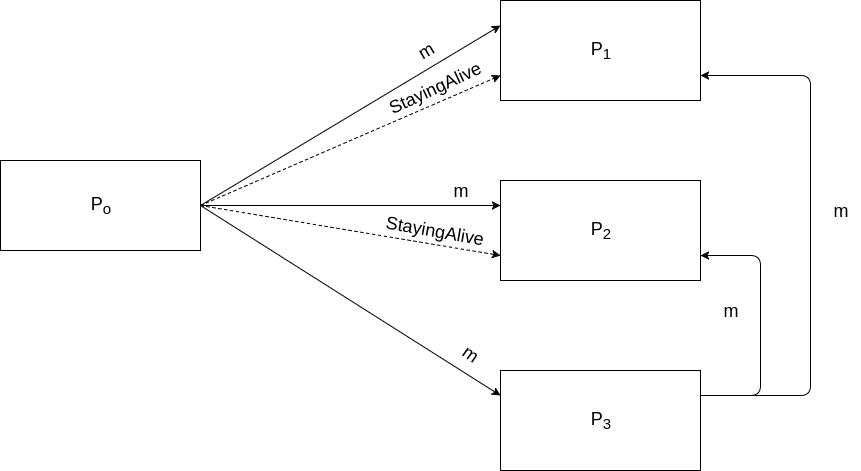
\includegraphics[width=\linewidth]{images/04-FIFO_RRB.png}
    \caption{Przykład działania algorytmu zgodnego rozgłaszania niezawodnego stosowanego w proponowanym systemie}
    \label{figure:systemdescription_fifo_rrb}
\end{figure}

Na rysunku \ref{figure:systemdescription_fifo_rrb} została przedstawiona sytuacja, w której proces $ P_o $ dokonujący rozgłaszania wiadomości $ m $, rozsyła najpierw tą wiadomość do węzłów $ P_1 $, $ P_2 $ oraz $ P_3 $, po czym wysyła komunikaty \texttt{StayingALive}, najpierw do $ P_1 $, potem do $ P_2 $, a następnie ulega awarii. Komunikat \texttt{StayingALive} nigdy nie dotrze do procesu $ P_3 $, dlatego ten po upłynięciu czasu oczekiwania na tą wiadomość dokona samoczynnego rozgłaszania wiadomości $ m $ do pozostałych procesów. W przypadku, gdyby proces $ P_o $ uległ awarii w trakcie rozsyłania wiadomości $ m $, ale udałoby mu się wysłać ją do co najmniej jednego poprawnego procesu, to proces(y) te nie otrzymałyby również komunikatu \texttt{StayingALive} i po określonym czasie również dokonałyby ponownego rozgłaszania tak, aby wszystkie poprawne procesy w końcu otrzymały rozgłaszaną wiadomość $ m $.

\subsection{Śledzenie zależności przyczynowych pomiędzy zapisami}

Zadanie ustalenia jaka wartość określonego klucza jest zgodna z modelem spójności przyczynowej bądź sekwencyjnej wymaga prześledzenia zależności przyczynowych pomiędzy operacjami zapisu mającymi miejsce w systemie. Oczywiście w lokalnym buforze entropii może istnieć wiele operacji zapisu dotyczących określonego klucza, jednak należy wybrać tę, która jest najświeższa (w rozumieniu definicji porządku przyczynowego z rozdziału \ref{chapter:replication}), a jednocześnie entropia zawiera jej pełen prefiks przyczynowy, tak aby kolejne odczyty zwracały wartość co najmniej tak samo świeżą jak poprzednie.

W celu realizacji wyżej postawionego zadania, każda wiadomość dotycząca operacji zapisu w systemie otrzymuje swój własny, unikalny zegar wektorowy, który jest następnie przesyłany zawsze w parze z tą wiadomością. Dzięki możliwości porównywania wartości zegarów wektorowych dwóch różnych wiadomości $ m_1 $, $ m_2 $ możliwe jest jednoznaczne stwierdzenie, że np. operacja zapisu zawarta w wiadomości $ m_1 $ zależy przyczynowo od operacji zapisu zawartej w wiadomości $ m_2 $ albo na odwrót, lub też, że obie operacje są zdarzeniami niezależnymi. W tym miejscu należy dokładnie określić, co rozumiane jest pod pojęciem zegarów wektorowych.

\subsubsection{Zegary logiczne}

% [MB] Przydałby się przypis

\textit{Zegarem logicznym} systemu rozproszonego nazywamy funkcję $ \mathcal{T}: \Lambda \rightarrow \mathcal{Y} $, odwzorowującą zbiór zdarzeń $ \Lambda $ w zbiór uporządkowany $ \mathcal{Y} $, taką że:
\begin{align*}
    (E \mapsto E') \Rightarrow (T(E) < T(E'))    
\end{align*}
gdzie < jest relacją porządku na zbiorze $ \mathcal{Y} $.

\textit{Zegarem wektorowym} nazywamy z kolei zegar logiczny, dla którego przeciwdziedzina funkcji $ \mathcal{T} $, oznaczana dalej dla odróżnienia przez $ \mathcal{T}^V $, jest zbiorem n-elementowych wektorów liczb naturalnych lub rzeczywistych. Oznacza to, że w systemie składającym się z n serwerów, każdy zegar wektorowy będzie zawierał n pozycji, gdzie każda z nich odpowiadać będzie dokładnie jednemu serwerowi. Dodatkowo, wartość na n-tej pozycji zegara logicznego oznacza wartość czasu wirtualnego, o którego upływie był świadomy serwer nadający wiadomości zegar wektorowy w odniesieniu do n-tego serwera systemu.

\subsection{Sekwencjonowanie i materializacja danych} \label{section:materialization}

% [MB] tytuł "Materializacja danych" lub "Sekwencjonowanie i materializacja danych". Wydaje mi się, że pojęcia "materializacja" i "sekwencjonowanie" (lub podobne) powinny być używane w taki sposób, jak w implementacji, tzn. materializacja - faktyczny zapis wartości do trwałego nośnika, sekwencjonowanie - proces nadawania numerów sekwencyjnych.
% [BK] poprawiłem nazewnictwo

Sekwencjonowanie jako proces zachodzący w systemie zostało już wspomniane wcześniej w niniejszym rozdziale. Odpowiada ono za nadawanie kolejnych numerów sekwencyjnych operacjom zapisu nadchodzącym do systemu, tj. dokonuje ich globalnego uszeregowania, zachowując jednocześnie porządek przyczynowy operacji. Przeprowadzaniem procesu sekwencjonowania zajmuje się jeden, wyróżniony serwer, zwany \textit{sekwencerem}. Ważne jest, aby w całym systemie (przy obecnej implementacji) istniał dokładnie jeden taki proces. Jeśli żaden z serwerów nie będzie pełnił roli sekwencera, to lokalne bufory entropii będą rosnąć, a dane nigdy nie osiągną spójności sekwencyjnej oraz nie zostaną zapisane do używanej wewnętrznie bazy danych. Jeśli z kolei nada się rolę sekwencera więcej niż jednemu serwerowi, wówczas przechowywane dane będą mogły stać się z czasem niespójne, ze względu na inne uszeregowanie zapisów generowane przez poszczególne sekwencery. Z powyższego wynika bezpośrednio problem, o którym szerzej traktuje sekcja \ref{subsection:sequencerfailures} rozdziału poświęconemu szczegółom implementacyjnym, tj. sekwencer jest newralgicznym punktem systemu, a od jego prawidłowej pracy zależy postęp całego przetwarzania, ponieważ tylko on może decydować o przejściu danych na poziom spójności sekwencyjnej.

\subsubsection*{Pseudokod procedury sekwencjonowania}

Zostaną teraz przedstawione pseudokody procedur obsługi wiadomości związanych z procedurą materializacji danych, procedury nadawania kolejnych numerów sekwencyjnych operacjom zapisu w systemie oraz procedury dokonującej materializacji (czyli zapisania danych z bufora entropii do wewnętrznie używanej bazy danych - backendu). W podanych pseudokodach zastosowano następujące oznaczenia:
\begin{itemize}
    \item \texttt{EntropyMessage} - oznacza typ wiadomości wymianianej pomiędzy serwerami w systemie, informującej o wystąpieniu nowego zdarzenia zapisu danych
    \item \texttt{IS\_SEQUENCER} - predykat prawdziwy wtedy i tylko wtedy gdy bieżący serwer pełni rolę sekwencera w systemie
    \item \texttt{can\_be\_delivered(MESSAGE, MATERIALIZE\_VC)} - procedura zwracająca odpowiedź prawda lub fałsz w zależności od tego, czy wiadomość MESSAGE może być już dostarczona przy założeniu, że wartość lokalnego zegara wektorowego zawarta jest w \texttt{MATERIALIZE\_VC}
    \item \texttt{synchronize} - operacja przepisania pozycji o większych wartościach z dwóch zegarów wektorowych, wynikiem jest nowy zegar wektorowy
    \item \texttt{broadcast} - operacja zgodnego rozgłaszania niezawodnego z zachowaniem porządku FIFO
    \item \texttt{copy} - operacja tworząca głęboką kopię danego obiektu (ang. \texttt{deep copy})
    \item \texttt{LAST\_MATERIALIZED\_SEQ\_NO} - numer ostatnio nadanego numeru sekwencyjnego
    \item \texttt{LAST\_MATERIALIZED\_CACHE\_NO} - numery sekwencyjne ostatnio nadawane operacjom aktualizacji w odniesieniu do poszczególnych kluczy
    \item \texttt{SEQUENCED\_MESSAGES\_VC} - bufor nadanych przez sekwencer numerów sekwencyjnych dla wiadomości, które nie mogą być jednak w danej chwili zmaterializowane na bieżącym węźle
    \item \texttt{MATERIALIZE\_VC} - wartość zegara wektorowego w momencie ostatnio przeprowadzanego procesu nadawania numerów sekwencyjnych (dotyczy sekwencera)
    \item \texttt{ENTROPY} - bufor entropii
    \item \texttt{length} - funkcja długości listy (podaje liczbę elementów listy będącej argumentem)
    \item \texttt{indexOf} - funkcja, której wartością jest numer (indeks) wskazanego elementu na podanej liście
\end{itemize}

Dodatkowo używane są skróty w nazwach składowych przekazywanych struktur: \texttt{VC} oznacza wartość zegara wektorowego, \texttt{SEQ\_NO} - numer sekwencyjny wiadomości (uaktualnienia), \texttt{CACHE\_NO} - numer sekwencyjny w odniesieniu do danego klucza, a \texttt{KEY} sam klucz, pod którym znajdują się dane.

\begin{lstlisting}[language=Pascal, caption=Pseudokod procedury próbującej dokonać sekwencjonowania w procesie sekwencera, mathescape=true]
procedure assignSequentialOrder(MESSAGE: EntropyMessage)
begin
    if IS_SEQUENCER and can_be_delivered(MESSAGE, MATERIALIZE_VC) then
    begin
        MAT_VC_ORDER := materializable_sequence(MATERIALIZE_VC)
        MATERIALIZE_VC := synchronize(MATERIALIZE_VC, MESSAGE.VC)
        broadcast MAT_VC_ORDER to all servers
    end
end
\end{lstlisting}

Procedura \texttt{assignSequentialOrder} jest wywoływana za każdym razem, gdy do systemu zosanie zgłoszone nowe żądanie zapisu danych. Sprawdza ona, czy bieżący proces jest sekwencerem oraz czy posiada pełen prefiks przyczynowy dla nowej wiadomości \texttt{MESSAGE}. Jeśli tak, to następuje przypisanie numerów sekwencyjnych wiadomościom w buforze entropii (procedura \texttt{materializable\_sequence}), zsynchronizowanie wartości lokalnego zegara wektorowego oraz rozesłanie do pozostałych serwerów właśnie wyznaczonego porządku sekwencyjnego dla wiadomości wraz z ich zegarami wektorowymi.

\begin{lstlisting}[language=Pascal, caption=Pseudokod funkcji konstruującej listę nowych numerów sekwencyjnych wiadomościom z bufora entropii, mathescape=true]
function materializable_sequence(STARTING_POINT: VectorClock, 
                                  SEQ_ACC: List[VectorClock], 
                                  EACH_KEY_ACC: Map[String, List[VectorClock]])
    : List[OrderTag]
var
    new_virtual_clock: VectorClock
    start_cache_no: Integer
    order_tags: List[OrderTag] = List()
    each_key_with_cache_no: List[(String, Integer, VectorClock)] = List()
begin
    if there is message MSG $ \in $ ENTROPY such that 
       can_be_delivered(MSG, STARTING_POINT) is true then
        begin
            new_virtual_clock = synchronize(STARTING_POINT, MSG.VECTOR_CLOCK)
            SEQ_ACC += MSG.VECTOR_CLOCK
            EACH_KEY_ACC[MSG.KEY] += MSG.VECTOR_CLOCK
            
            materializable_sequence(new_virtual_clock, SEQ_ACC, EACH_KEY_ACC)
        end
    else
        begin
            for each KEY, VECTOR_CLOCKS in EACH_KEY_ACC
            begin
                start_cache_no := LAST_MATERIALIZED_CACHE_NO(KEY) + 1
                for i := start_cache_no to start_cache_no + length(VECTOR_CLOCKS),
                    j := 0 to length(VECTOR_CLOCKS) do
                begin
                    each_key_with_cache_no += (KEY, i, VECTOR_CLOCKS[j])
                end
            end
            for each (KEY, CACHE_NO, VECTOR_CLOCK) in each_key_with_cache_no do
            begin
                order_tags += OrderTag(
                    VECTOR_CLOCK, 
                    indexOf(VECTOR_CLOCK, SEQ_ACC) + LAST_MATERIALIZED_SEQ_NO + 1, 
                    CACHE_NO, 
                    KEY
                )
            end
        end
    end
    return order_tags
end
\end{lstlisting}

Funkcja \texttt{materializable\_sequence} na podstawie aktualnej zawartości bufora entropii oraz wartości lokalnego zegara wektorowego nadaje nowe numery sekwencyjne wiadomościom, dla których posiada pełne prefiksy przyczynowe w lokalnym buforze entropii. Wartością tej funkcji jest lista zawierająca numery sekwencyjne nadane wiadomościom wraz z przypisanymi do nich wartościami zegarów wektorowych.

\begin{lstlisting}[language=Pascal, caption=Pseudokod obsługi wiadomości zawierającej porządek sekwencyjny dla operacji zapisów w systemie, mathescape=true]
on receive(MAT_VC_ORDER: List(VC, SEQ_NO, CACHE_NO, KEY))
begin
    for each ELEMENT of MAT_VC_ORDER sorted by SEQ_NO
    begin
        SEQUENCED_MESSAGES_VC += (VC, SEQ_NO, CACHE_NO, KEY)
        process(VC, SEQ_NO, CACHE_NO, KEY)
    end
end
\end{lstlisting}

Otrzymując listę z nowymi numerami sekwencyjnymi, serwer dodaje je do zbioru \texttt{SEQUENCED\_MESSAGES\_VC} oraz wywołuje dla każdego nowego numeru sekwencyjnego procedurę \texttt{process}, której efektem może być dokonanie materializacji danych w wewnętrznie używanej bazie danych.

\begin{lstlisting}[language=Pascal, caption=Pseudokod procedury obsługi wiadomości informującej o nowym zapisie w systemie, mathescape=true]
on receive(MSG(KEY, VALUE, VC): EntropyMessage)
begin
    ENTROPY += MSG
    for each ELEMENT of copy(SEQUENCED_MESSAGES_VC) sorted by SEQ_NO
    begin
        process(ELEMENT.VC, ELEMENT.SEQ_NO, ELEMENT.CACHE_NO, ELEMENT.KEY)
    end
end
\end{lstlisting}

W sytuacji, w której do systemu nadejdzie nowe żądanie zapisu, jest ono dodawane do lokalnego bufora entropii. Nowa wiadomość typu \texttt{EntropyMessage} być może uzupełni prefiks przyczynowy innych wiadomości w lokalnym buforze entropii, dla których jednocześnie w zbiorze \texttt{SEQUENCED\_MESSAGES\_VC} mogą być już przechowywane numery sekwencyjne. Z tego powodu następnie przetwarzany jest każdy element tego zbioru w nadziei, że uda się dokonać materializacji nowych danych.

\begin{lstlisting}[language=Pascal, caption=Pseudokod procedury próbującej dokonać materializacji o ile jest to możliwe, mathescape=true]
procedure process(VC, SEQ_NO, CACHE_NO, KEY)
begin
    if LAST_MATERIALIZED_SEQ_NO is SEQ_NO - 1
    and MSG(VC, ...) $ \in $ ENTROPY then
        materialize(MSG(VC, ...), SEQ_NO, CACHE_NO)
    end
end
\end{lstlisting}

Sama materializacja może dokonać się tylko wówczas, jeśli wiadomość, której zapis ma być materializowany, posiada kolejny numer sekwencyjny względem numeru sekwencyjnego ostatnio materializowanej wiadomości oraz sama wiadomość z odpowiednią wartością zegara wektorowego (pełni on rolę unikalnego identyfikatora wiadomości w systemie) znajduje się w lokalnym buforze entropii. Spełnienie tego warunku oznacza dokonanie właściwej materializacji w procedurze \texttt{materialize}.

\begin{lstlisting}[language=Pascal, caption=Pseudokod procedury materializacji wartości na danym węźle, mathescape=true]
procedure materialize(MESSAGE(KEY, VALUE, VC), SEQ_NO, CACHE_NO)
begin
    save MESSAGE to backend
    LAST_MATERIALIZED_SEQ_NO := SEQ_NO
    LAST_MATERIALIZED_CACHE_NO(KEY) := CACHE_NO
    ENTROPY $ \textbackslash $= MESSAGE
    SEQUENCED_MESSAGES_VC $ \textbackslash $= (VC, SEQ_NO, CACHE_NO, KEY)
end
\end{lstlisting}

Procedura \texttt{materialize} dokonuje właściwej materializacji danych w wewnętrznie używanej przez system bazie danych (ang. \textit{backend}). Najpierw zapisuje uaktualnienie danych zawarte w wiadomości \texttt{MESSAGE} do bazy danych. Następnie następuje aktualizacja wartości numeru sekwencyjnego ostatnio materializowanej wiadomości: globalnego oraz w odniesieniu do konkretnego klucza. Wiadomość \texttt{MESSAGE} jest usuwana z lokalnego bufora entropii, a ze zbioru \texttt{SEQUENCED\_MESSAGES\_VC} usuwa się informację o numerze sekwencyjnym dla unikalnej wartości zegara wektorowego \texttt{VC}.

% TODO przykłady dla cache, causal i pram
\subsection{Konstrukcja wartości zgodnych z poszczególnymi modelami danocentrycznymi} \label{section:value_construction}

Kiedy do serwera przychodzi żądanie pobrania wartości zgodnej z określonym modelem danocentrycznym musi on potrafić skonstruować odpowiedź spełniającą oczekiwany przez użytkownika poziom spójności. Niniejszy punkt opisuje w jaki sposób i na podstawie jakich danych następuje generacja odpowiedzi przez serwer proponowanego systemu. 

\subsubsection{Spójność sekwencyjna}

W przypadku żądania pobrania danych spójnych sekwencyjnie pod określonym kluczem, serwer odpytuje wewnętrzną bazę danych (ang. \textit{backend}) i podaje użytkownikowi w odpowiedzi to, co samemu otrzymał z bazy danych. Może to być konkretna wartość lub wartość specjalna \texttt{None}, oznaczająca, że podany klucz nie istnieje w bazie danych odpytywanego serwera.

W przypadku, w którym konstruując odpowiedź dla modelu spójności podręcznej, przyczynowej lub PRAM okaże się, że serwer nie jest w stanie podać konkretnej wartości, następuje automatyczne pobranie wartości spójnej sekwencyjnie --- także wtedy, gdy bufor entropii jest pusty (bowiem wartość spójna sekwencyjnie spełnia także wszystkie wymienione warunki spójności).

\subsubsection{Spójność podręczna}

Konstruując wartość zgodną z modelem spójności podręcznej system sprawdza, czy nie otrzymał już numerów sekwencyjnych dla wiadomości, które obecnie wciąż znajdują się w entropii. Taka sytuacja może mieć miejsce w przypadku, gdy serwer otrzymał numer(y) sekwencyjne dla pewnych operacji zapisu, ale nie otrzymał jeszcze numerów sekwencyjnych dla jakiś wcześniejszych operacji zapisu. Wówczas serwer nie może dokonać zapisu do wewnętrznej bazy danych, ponieważ brak mu poprzedzających numerów sekwencyjnych, a jednocześnie może posiadać w entropii wiadomości, których numery sekwencyjne także posiada. W takim przypadku, w odniesieniu do jednego klucza, serwer może posiadać zarówno wiadomości zapisu w buforze entropii, jak i ich numery sekwencyjne, tak więc może odpowiedzieć klientowi wartością, która jest spójna w sensie spójności podręcznej, a jednocześnie nie została jeszcze przeniesiona do wewnętrznej bazy danych (backendu). % Tak właśnie działa wyznaczanie wartości spójnych podręcznie w proponowanym systemie.

\subsubsection{Spójność przyczynowa}

Wartość spójna przyczynowo konstruowana jest na podstawie zawartości bufora entropii oraz wartości lokalnego zegara wektorowego w momencie ostatnio przeprowadzonego procesu materializacji. Serwer szuka w swoim buforze entropii wiadomości z możliwie największym znacznikiem czasowym (w formie zegara wektorowego nadanego w momencie rozgłaszania tej wiadomości przez inny serwer), dla której posiada jednocześnie pełny prefiks przyczynowy w buforze entropii. Znaleziona wiadomość dotyczy zapisu pod określony klucz wartości $ v $, i to właśnie $ v $ jest zwracana jako odpowiedź.

\subsubsection{Spójność PRAM}

W przypadku spójności PRAM serwer pobiera najnowszą wiadomość ze swojego zbioru entropii (najnowszą w sensie ostatnio otrzymaną), dotyczącą żądanego klucza. Wiadomość ta dotyczy zapisu wartości $ v $ pod określony klucz i to właśnie $ v $ jest wartością zwracaną klientowi. Dzieje się tak dlatego, że rozgłaszanie wiadomości o kolejnych operacjach zapisu w systemie odbywa się za pomocą mechanizmu zgodnego rozgłaszania niezawodnego zachowującego porządek FIFO. Wynika z tego, że kolejne operacje zapisu przyjęte przez jeden węzeł będą w takiej samej kolejności przyjmowane przez inne węzły, co oznacza zachowanie spójności PRAM.

\subsection{Realizacja gwarancji sesji}

Istnieje wiele protokołów służących zapewnieniu, że implementowany system będzie dawał użytkownikowi możliwość wyboru gwarancji sesji (jednej lub więcej), z którymi ma zostać wykonana określona operacja dostępu do danych (odczyt lub zapis). Przykładowymi rozwiązaniami są:
\begin{itemize}
    \item protokół logiczny
    \item protokół VsSG
    \item protokół VcSG
    \item protokół VoSG
\end{itemize}

Protokół logiczny przydatny jest w rozważaniach teoretycznych, lecz nie jest implementowany w praktyce, ponieważ zakłada przesyłanie w każdym żądaniu od klienta do serwera całego zbioru operacji niezbędnych do wykonania wcześniej od operacji zawartej w żądaniu. Wraz z postępem przetwarzania rozmiar przesyłanych komunikatów byłby coraz większy, co w końcu mogłoby uniemożliwić dalszą pracę systemu.

Kolejne proponowane rozwiązanie to protokół korzystający z wektorów wersji opartych na operacjach wykonanych na poszczególnych serwerach, nazywany VsSG. Jest to jednocześnie rozwiązanie zaimplementowane w proponowanym systemie. Jednak zanim zostanie ono dokładnie opisane, należy wyjaśnić pojęcie wektora wersji. Protokoły VcSG oraz VoSG zostaną tylko krótko opisane dla kompletności rozważań.

\subsubsection{Wektory wersji} \label{subsection:version_vector}

% [MB] Przypis na temat wektorów wersji

\textit{Wektorem wersji} nazywamy sekwencję liczb, z których każda odpowiada zarejestrowanej liczbie zapisów wykonanych na serwerze związanym z pozycją tej liczby w wektorze wersji. Koncepcyjnie są one oparte na idei zegarów wektorowych, zapewniając (tak jak zegary wektorowe) unikalną identyfikację zapisów w systemie. Zastępują one zbiory operacji używane w protokole logicznym, umożliwiając efektywną reprezentację wymagań dotyczących przeprowadzanej w systemie operacji. W przypadku proponowanego systemu w roli wektorów wersji zostały użyte zegary wektorowe - informacja w nich zawarta jest tożsama z wektorem wersji, ponadto zegary wektorowe zostały zaimplementowane w pierwszej kolejności dla śledzenia zależności przyczynowych pomiędzy operacjami zapisu w systemie. Ich ponowne wykorzystanie było więc naturalną decyzją.

Formalnie, można zapisać wektor wersji w następujący sposób:
\begin{align*}
    V = [v_1 v_2 ... v_N]
\end{align*}
gdzie N jest liczbą serwerów, klientów bądź współdzielonych obiektów w systemie, w zależności od używanego protokołu. Dodatkowo, dla wektorów wersji definiuje się relację dominacji w następujący sposób:
\begin{align*}
    \forall{i}: V_1[i] \geqslant V_2[i] 
\end{align*}

\subsubsection{Protokół VsSG}

Jak już wspomniano, protokół VsSG wykorzystuje wektory wersji oparte na serwerach, zdefiniowane następująco:
\begin{align*}
    V_S = [v_1 v_2 ... v_{N_S}]
\end{align*}
gdzie $ v_i $ oznacza liczbę zapisów wykonanych przez serwer $ S_i $ a $ N_S $ jest ogólną liczbą serwerów w systemie.

W dalszej części rozdziału zostaną przedstawione pseudokody procedur realizujących protokół VsSG, jednak w pierwszej kolejności należy objaśnić występujące w nich oznaczenia:
\begin{itemize}
    \item $ O_{S_j} $ to zbiór operacji zapisu wykonanych przez serwer $ S_j $
    \item $ W_{C_i} $ to zbiór operacji zapisu wykonanych przez klienta $ C_i $
    \item $ R_{C_i} $ to zbiór operacji zapisu, których efekty zostały (częściowo) odczytane przez klienta $ C_i $
    \item $ <op, SG> $ to żądanie wykonania operacji $ op $ z uwzględnieniem gwarancji sesji ze zbioru $ SG $
    \item $ <op, W> $ to żądanie wykonania operacji $ op $ wysyłane do serwera, a $ W $ to zbiór operacji wymaganych do wykonania operacji $ op $
    \item $ <op, res, W> $ to odpowiedź serwera składająca się z wyniku operacji $ op $ zapisanego w $ res $ oraz zbioru operacji będącego wynikiem wykonania $ op $
operacji op
\end{itemize}

Zostaną teraz przedstawione pseudokody procedur wysyłania żądania przez klienta do serwera, przetwarzania żądania po stronie serwera oraz przetwarzania odpowiedzi od serwera po stronie klienta.

\begin{lstlisting}[language=Pascal, caption=Pseudokod procedury wysyłania żądania przez klienta w protokole VsSG, mathescape=true]
W  $ \leftarrow $ 0
if (iswrite(op) and MW $ \in $ SG) or (not iswrite(op) and RYW $ \in $ SG) then
    W $ \leftarrow $ max(W, W$_{C_i} $)
end if
if (iswrite(op) and WFR $ \in $ SG) or (not iswrite(op) and MR $ \in $ SG) then
    W $ \leftarrow $ max(W, R$_{C_i} $)
end if
send<op, W> to S$_j $
\end{lstlisting}

Wyjaśnić należy użyte w powyższym kodzie wywołania funkcji \texttt{iswrite}, \texttt{max} oraz \texttt{send}. Funkcja \texttt{iswrite} przyjmuje jako argument operację $ op $, a jej wartością jest prawda lub fałsz w zależności od tego czy $ op $ jest operacją zapisu (prawda) czy nie (fałsz). Funkcja \texttt{max} pobiera dwa wektory na wejściu a jej wartością jest wektor składający się z maksymalnych wartości na poszczególnych pozycjach wektorów wejściowych. Operacja \texttt{send} wysyła żądanie od klienta do serwera.

Zanim żądanie z podanymi gwarancjami sesji zostanie wysłane do serwera, należy skonstruować wymagany, minimalny wektor wersji, którego wartość musi zdominować (w sensie przedstawionym w punkcie \ref{subsection:version_vector}) wektor przechowywany na serwerze, aby ten mógł wykonać żądaną operację. Wektor ten nazywany jest tu $ W $ i konstruowany poczynając od wektora zerowego. Następnie, jeśli żądamy wykonania zapisu z gwarancją monotonicznych zapisów (\textit{Monotonic Writes}) lub odczytu z gwarancją odczytu własnych zapisów (\textit{Read Your Writes}), to do wektora $ W $ podstawiamy wartość wektora z operacjami zapisów wykonanych przez klienta (tak, aby kolejny zapis nastąpił na wszystkich serwerach w sposób monotoniczny lub by odczyt nastąpił po własnych zapisach). Jeśli z kolei żądaną operacją jest odczyt z zachowaniem gwarancji monotonicznych odczytów (\textit{Monotonic Read}) lub zapis z zachowaniem gwarancji zapisów po odczytach (\textit{Writes Follow Reads}), to należy skonstruować wektor wersji uwzględniający operacje zapisu, których efekty zostały odczytane przez klienta (to znaczy operacje zawarte w wektorze $ R_{C_i} $). Na końcu następuje wysłanie żądania do serwera (operacja \texttt{send}).

Następnie zostanie przedstawiony pseudokod obsługi żądania po stronie serwera.

\begin{lstlisting}[language=Pascal, caption=Pseudokod procedury obsługi żądania po stronie serwera w protokole VsSG, mathescape=true]
while (not V$_{S_j} \geq $ W) do
    wait()
end while
wykonaj operacje op i zapisz wyniki w res
if iswrite(op) then
    V$_{S_j}$[j] $ \leftarrow $ V$_{S_j}$[j] + 1
end if
send <op, res, V$_{S_j}$> to C$_i$
\end{lstlisting}

Klient $ C_i $ wysłał żądanie wykonania operacji $ op $ do serwera $ S_j $. Serwer po otrzymaniu żądania wstrzymuje się z wykonaniem operacji aż do momentu, w którym jego wektor wersji nie zdominuje wektora wersji przesłanego w żądaniu (w tym czasie serwer może obsługiwać inne żądania). Kiedy tak się stanie, serwer wykonuje żądaną operację $ op $, a jej wyniki zapisuje w $ res $. Dodatkowo, jeśli żądaną operacją był zapis, zwiększa wartość swojego wektora wersji na pozycji odpowiadającej jemu samemu o 1 (wykonał jeden nowy zapis). Na końcu następuje wysłanie odpowiedzi do klienta za pomocą funkcji \texttt{send}.

W oryginale protokół VsSG posiada także procedurę synchronizacji obrazów historii pomiędzy serwerami tak, aby ich wektory wersji uwzględniały zmiany poczynione na innych węzłach. W przypadku proponowanego systemu synchronizacja następuje samoczynnie poprzez rozgłaszanie komunikatów o operacjach  Pseuu zgłaszanych systemowi do wszystkich węzłów. Serwer odbierając taki komunikat aktualizuje swój wektor wersji (którym jest, jak powiedziano wcześniej, lokalny zegar wektorowy).

Następnym punktem jest przedstawienie kodu procedury przertwarzania odpowiedzi od serwera po stronie klienta.

\begin{lstlisting}[language=Pascal, caption=Pseudokod procedury obsługi odpowiedzi od serwera po stronie klienta w protokole VsSG, mathescape=true]
if iswrite(op) then
    W$_{C_i} \leftarrow $ max(W$_{C_i}$, W)
else
    R$_{C_i} \leftarrow $ max(R$_{C_i}$, W)
end if
deliver <res>
\end{lstlisting}

Otrzymując odpowiedź, klient aktualizuje zbiory operacji $ W_{C_i} $ albo $ R_{C_i} $ w zależności od tego, czy wykonana operacja była zapisem czy odczytem danych, po czym dostarcza odpowiedź użytkownikowi (operacja \texttt{deliver}).

\subsubsection{Protokół VcSG}

Protokół ten korzysta z wektorów wersji opartych na klientach:
\begin{align*}
    V_C = [v_1 v_2 ... v_{N_C}]    
\end{align*}
gdzie $ v_i $ oznacza liczbę zapisów zleconych przez klienta $ C_i $, a $ N_C $ jest ogólną liczbą klientów w systemie.

Protokół ten opiera się na założeniu, że operacje pochodzące od poszczególnych klientów muszą być globalnie uporządkowane.

\subsubsection{Protokół VoSG}

Protokół ten korzysta z wektorów wersji opartych na obiektach:
\begin{align*}
    V_O = [v_1 v_2 ... v_{N_O}]
\end{align*}
gdzie $ v_i $ oznacza liczbę zapisów wykonanych na obiekcie $ x_i $, a $ N_O $ jest ogólną liczbą współdzielonych obiektów w systemie.

Istotą tego protokołu jest zapewnienie, że operacje wykonywane na tych samych obiektach muszą być globalnie uporządkowane dla zachowania unikalności wektorów wersji.

\section{Zagadnienie podziału danych (ang. \textit{sharding})}

Wiele współczesnych rozproszonych baz danych oferuje możliwość korzystania z mechanizmu \textit{shardingu} danych, tj. podziału przechowywanych danych pomiędzy węzły. Dzięki temu rozwiązaniu węzły nie przechowują kopii całego zbioru danych, ale tylko wybrane jego części, co z kolei ułatwia skalowanie bazy danych. Mechanizm ten obecny jest więc w systemach o budowie podobnej do rozwiązania proponowanego w niniejszej pracy, mógłby być zatem zaimplementowany także w nim, aby każdy z serwerów przechowywał wartości tylko części kluczy. Zagadnienie to stanowi odrębny obszar problematyki replikacji danych, mogący rodzić nowe problemy związane z zachowaniem spójności bazy danych oraz wymagający rozwiązań implementacyjnych w zakresie dostępu do danych (nie będących już dostępnymi na każdym węźle). Niniejsza praca skupia się z kolei na umożliwieniu dostępu do danych z określonym poziomem spójności, co jest osobnym zagadnieniem oraz stanowi powód, dla którego zagadnienie to pozostawiono otwartym w proponowanym systemie. Aktualna implementacja nie wspiera podziału danych pomiędzy węzły, natomiast nie blokuje możliwości późniejszego rozwijania systemu właśnie w tym kierunku.
